\section[User-experience e visualizzazione dei dati]{User-experience e
visualizzazione\\dei dati}

Per fornire all'utente un'interfaccia grafica semplice e intuitiva si è deciso
di utilizzare gli eventi JavaScript per accompagnare l'utente in una procedura
guidata per l'inserimento dei parametri di ricerca. Tutto il codice JavaScript
(dove, per comodità, si fa uso anche della libreria jQuery) è stato inserito nel
file \code{dati-storici.js}.

In particolare, la pagina mostra inizialmente una \textit{drop-down list} dove
l'utente può selezionare la provincia di suo interesse tra tutte quelle di cui
sono disponibili dei dati. Una volta selezionata la provincia, il codice
JavaScript effettua una richiesta POST in tecnologia AJAX a
\code{getYearRange.php}, che esegue una query SQL sul database e ritorna, in
formato JSON, il range massimo di anni per cui sono disponibili misurazioni per
la provincia selezionata \idest{il primo e l'ultimo anno presenti nella tabella
\code{historical\_data}}. Questo range è utilizzato dal JavaScript per riempire
un'altra drop-down list --- quella dove l'utente può selezionare l'anno iniziale
per il periodo di interesse, che viene mostrata solo dopo che la richiesta POST
si è conclusa (inizialmente nascosta) --- con tutti gli anni compresi nel range
(estremi inclusi). In tal modo, possiamo garantire che l'utente non possa
scegliere range di anni troppo grandi che conterrebbero anni senza misurazioni e
complicherebbero inutilmente la visualizzazione dei dati.

Quindi, quando l'utente seleziona l'anno iniziale del periodo di suo interesse,
l'applicazione mostra una terza drop-down list nascosta per selezionare l'anno
di fine. Dopo che l'utente ha selezionato anche l'anno di fine, il codice
JavaScript invia una richiesta AJAX POST a \code{getHistoricalData.php} che
preleva i dati richiesti dalla tabella \code{historical\_data} e li ritorna in
formato JSON.

Infine, attraverso un'altra richiesta AJAX POST, questa volta a
\code{getDevicesByCity.php}, viene prelevata la lista di tutte le stazioni di
monitoraggio presenti nella provincia selezionata e viene inserita in un'altra
drop-down list che consente di filtrare i dati per stazione. Viene quindi
mostrata anche l'ultima drop-down list che consente di filtrare i dati per
inquinante: in questa lista vengono inseriti solo gli inquinanti per i quali
sono disponibili dati per la provincia o stazione selezionata, in modo che
l'utente non possa selezionare inquinanti per i quali non sono presenti
misurazioni.

In Figura \ref{fig:ux} è possibile vedere un esempio di compilazione di tutte
le drop-down list da parte dell'utente.

\begin{figure}[htb]
	\centering
	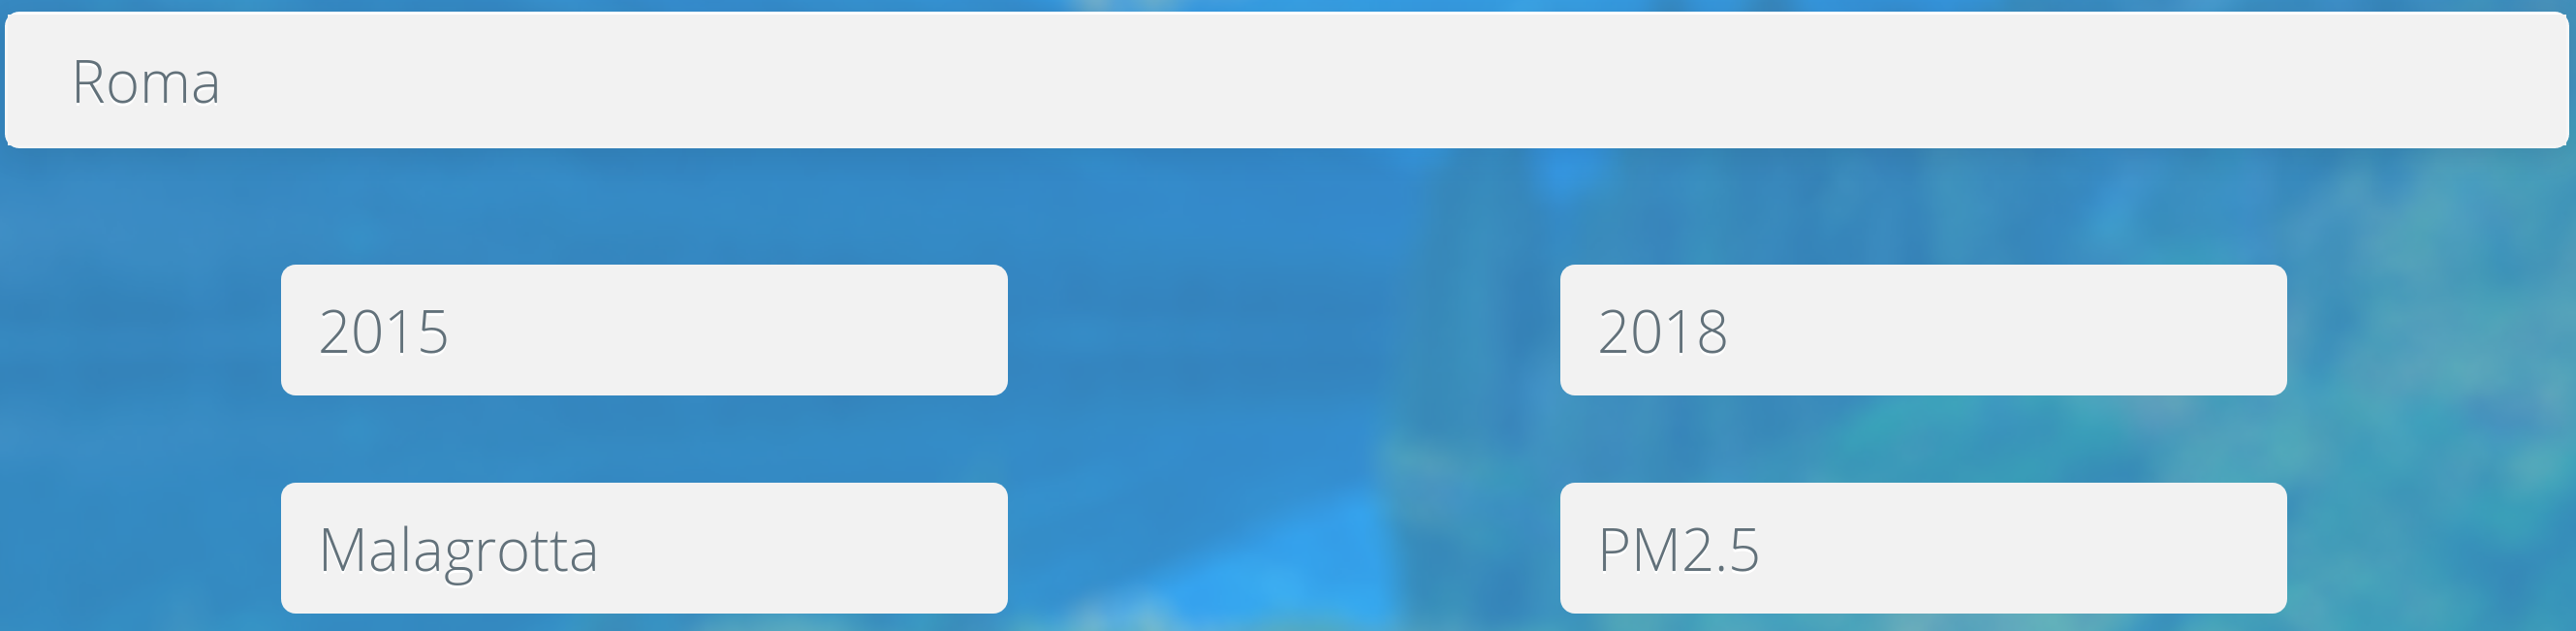
\includegraphics[width=\textwidth]{img/ux}
	\caption{Esempio di compilazione delle drop-down list che costituiscono
	l'interfaccia grafica della pagina.}\label{fig:ux}
\end{figure}

Per quanto riguarda la visualizzazione dei dati si è deciso di dividerla in due
parti: in una prima parte viene mostrata una tabella dove, per ogni anno e per
ogni quarto di anno, sono presentati: il maggior inquinante rilevato nell'aria,
relativamente al suo limite di riferimento; l'indice IQA percentuale calcolato
sul maggior inquinante (con relativo cromatismo mostrato con un piccolo cerchio
colorato); la variazione rispetto allo stesso quarto dell'anno precedente e di
due anni precedenti dell'IQA in termini percentuali (colorata di rosso se
positiva e di verde se negativa).

Sotto questa tabella viene anche mostrata la media percentuale dell'IQA per il
primo anno del range selezionato \idest{la media percentuale dell'IQA per i 4
quarti d'anno che compongono l'anno iniziale selezionato dall'utente} e per
l'ultimo anno del range. Quindi viene dato un giudizio globale (Migliorato,
Peggiorato o Invariato) basato sulla differenza tra queste due medie.

Qualora siano presenti dei buchi nei dati, questi dovranno comunque comparire in
tabella mostrando un trattino per indicare che per tale anno o periodo non sono
disponibili misurazioni. Questo permette di avere una tabella uniforme dove tra
una riga e l'altra c'è sempre la differenza di un solo quarto di anno.

La funzione che si occupa di generare il codice HTML per mostrare la tabella è
\code{getTableInnerHTML()}.

Un esempio di tabella, per la provincia di Milano per il periodo 2015--2019, è
mostrato in Figura \ref{fig:datatable}. Si noti come dalla tabella si può
facilmente dedurre che:
\begin{itemize}
	\item complessivamente, la qualità dell'aria è mediocre: l'IQA varia tra
		l'\(83\%\) e il \(176\%\), tenendosi il più delle volte sopra il
		\(100\%\);
	\item durante l'autunno e l'inverno (Q1 e Q4) l'inquinante maggiormente
		presente è il \(\chem{PM2.5}\) mentre durante la primavera e
		l'estate (Q2 e Q3) il più presente è l'\(\chem{O_3}\). Questo è
		in linea con quanto previsto, infatti le maggiori attività
		dell'industria e il più intenso traffico veicolari nelle città
		durante le stagioni fredde contribuiscono a far aumentare il
		particolato sottile nell'aria, mentre con il caldo e il maggior
		irraggiamento solare del periodo estivo si hanno le condizioni
		per attivare i processi chimico-fisici che portano alla
		formazione dell'ozono troposferico a partire dagli ossidi di
		azoto;
	\item nel corso degli anni, la qualità dell'aria a Milano è
		progressivamente migliorata: nei primi anni sono presenti molti
		cerchi rossi (qualità scadente) mentre non sono presenti negli
		ultimi due anni; inoltre le variazioni dell'IQA mostrano
		prevalentemente decrementi (verde) con pochi incrementi (rosso).
		La stessa informazione si può ricavare dal giudizio globale in
		fondo alla tabella.
\end{itemize}

\begin{figure}[htp]
	\centering
	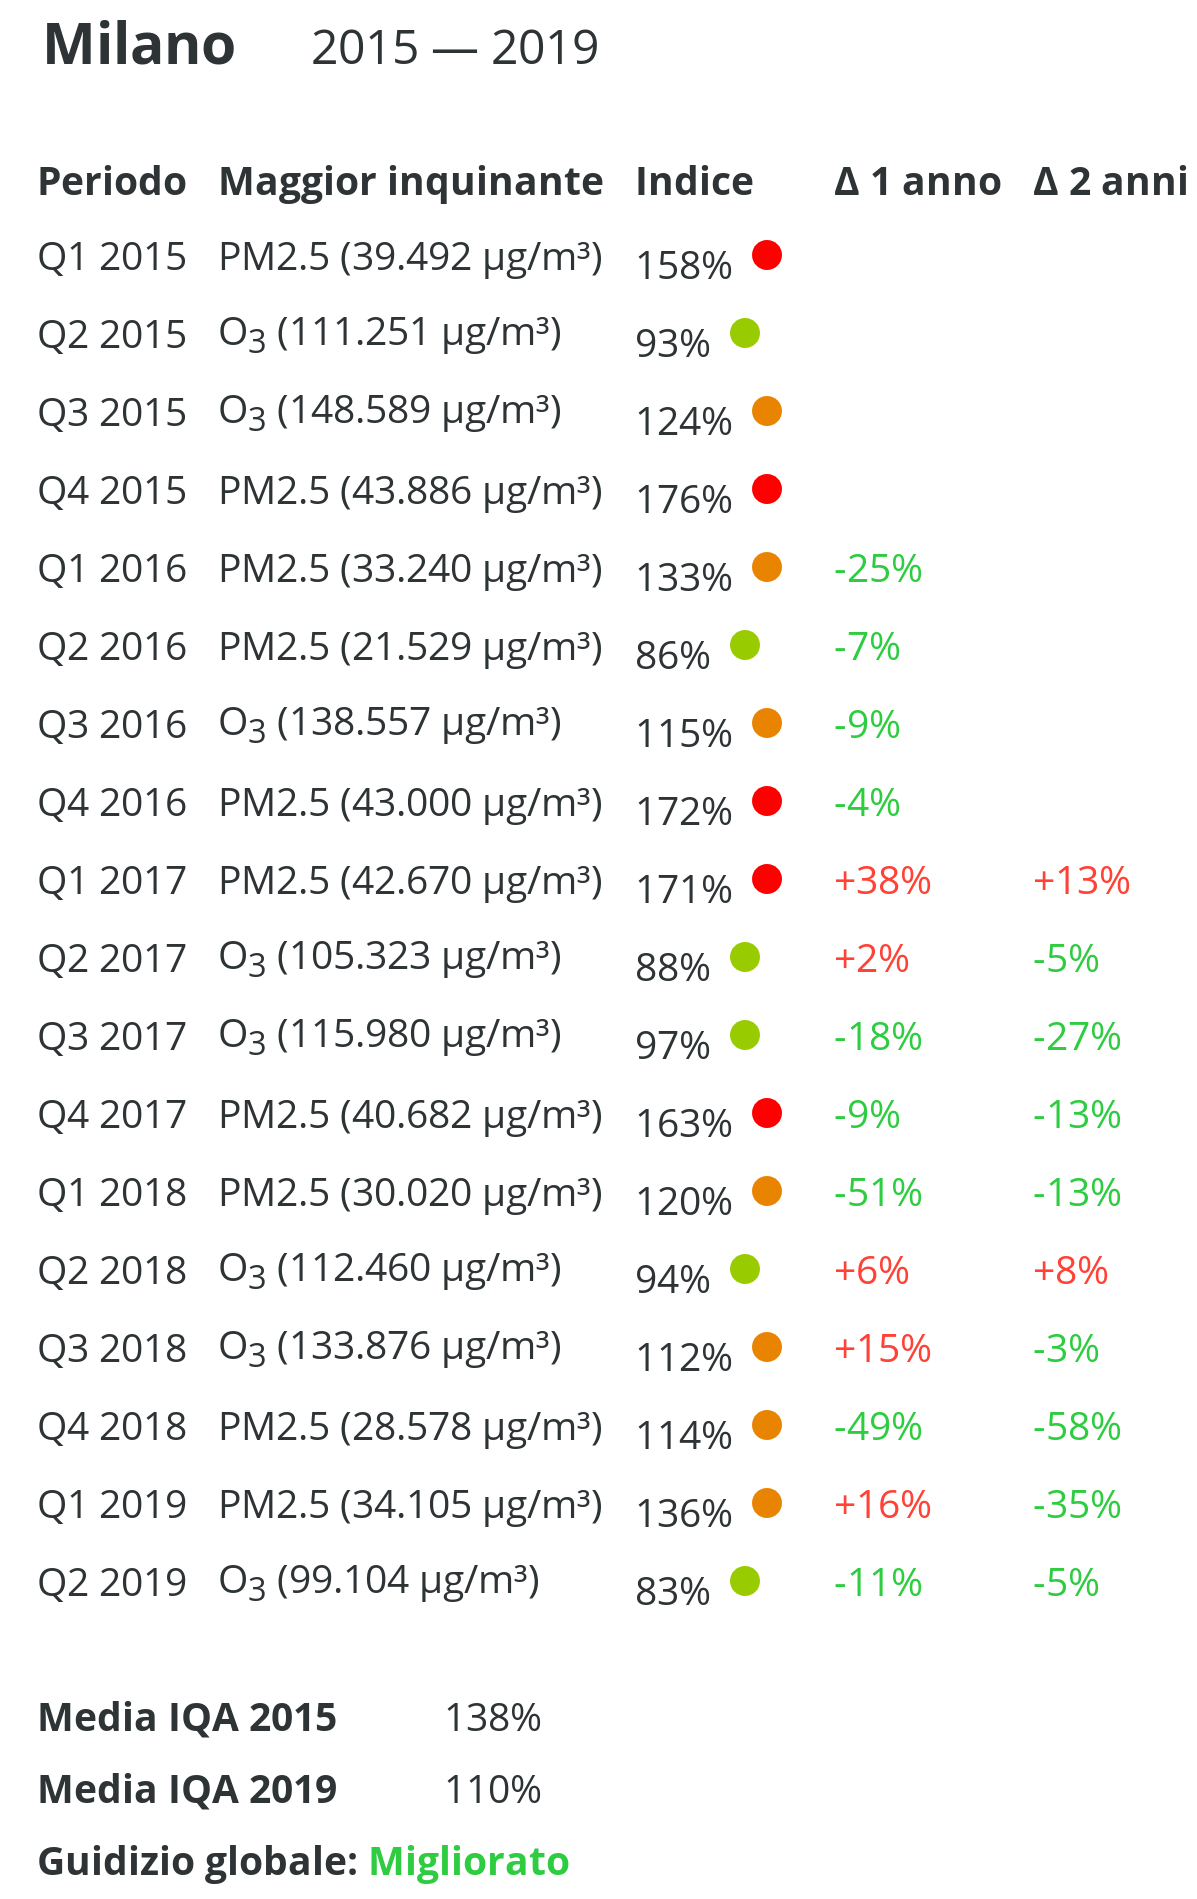
\includegraphics[width=0.7\textwidth]{img/datatable}
	\caption{Tabella della provincia di Milano per il periodo
	2015--2019.}\label{fig:datatable}
\end{figure}

Sotto alla tabella è mostrato anche un grafico dove viene illustrato l'andamento
di ogni inquinante (ogni linea corrisponde a un inquinante). Dal grafico,
realizzato con la libreria Google Charts, è possibile individuare immediatamente
trend e oscillazioni nella concentrazione degli inquinanti nell'aria.

La funzione che si occupa di inizializzare il grafico e inserire i dati è
chiamata \code{showGraphData()}.

In Figura \ref{fig:graph} è mostrato il grafico della provincia di Pisa per gli
anni 2014--2019. Si nota facilmente che:
\begin{itemize}
	\item l'ozono troposferico (\(\chem{O_3}\)) è in un trend leggermente
		rialzista, ed è maggiormente presente nei periodi caldi;
	\item il biossido di azoto (\(\chem{NO_2}\)) segue un trend ribassista,
		ed è maggiormente presente nei periodi freddi con l'incremento
		del traffico veicolare;
	\item la concentrazione degli altri inquinanti è generalmente rimasta
		invariata nel tempo e mostrano dei picchi durante il periodo
		invernale.
\end{itemize}

\begin{figure}[htp]
	\centering
	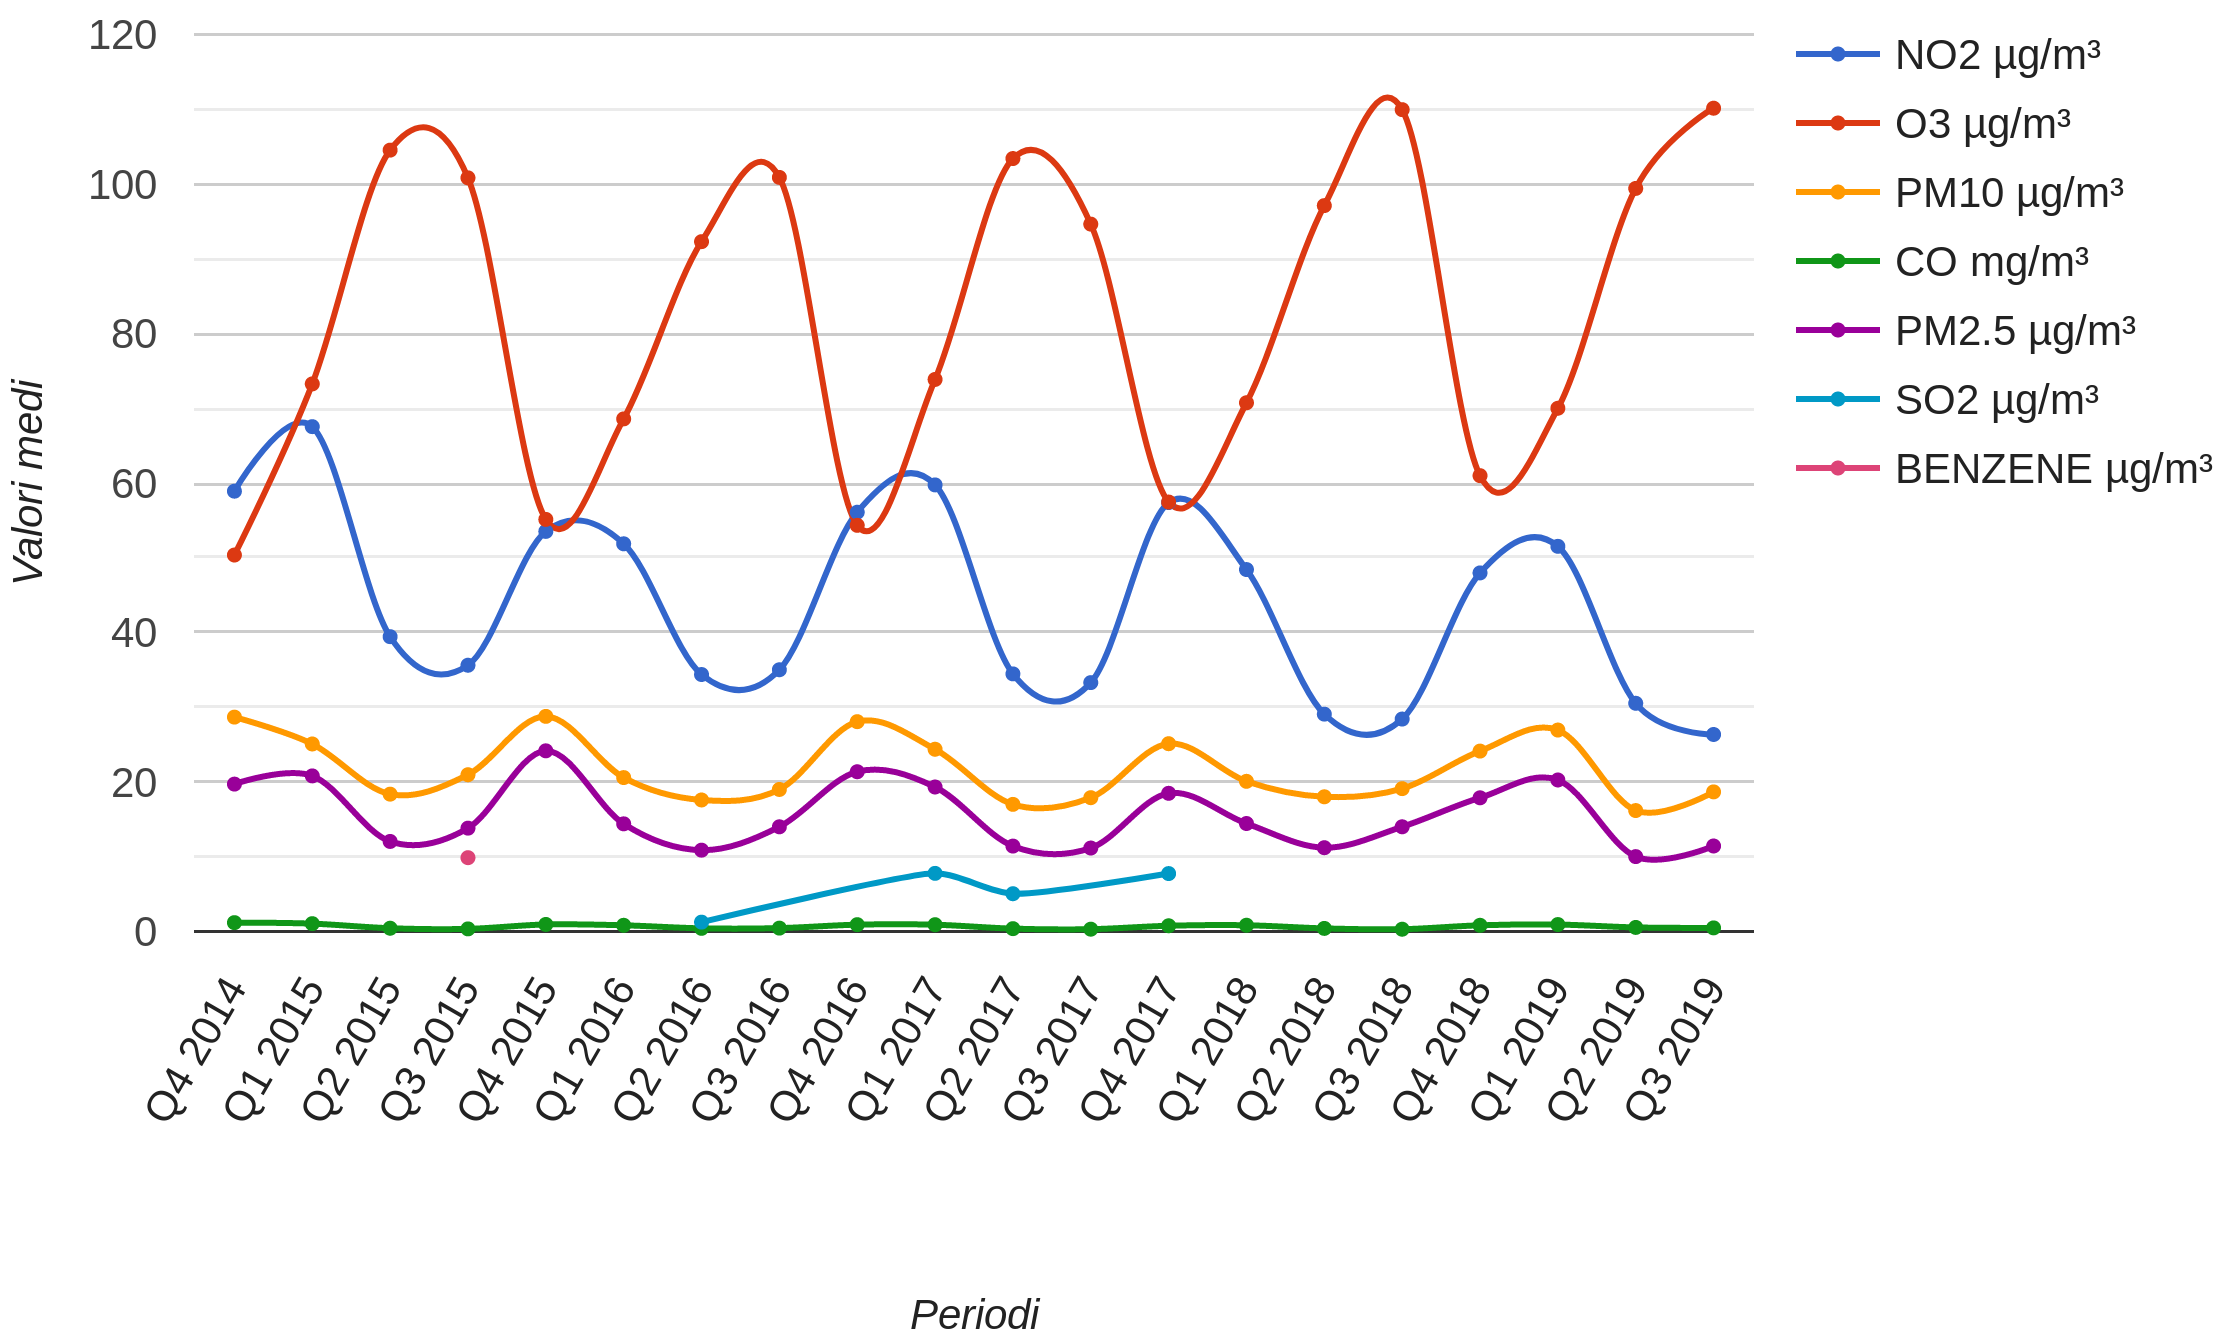
\includegraphics[width=\textwidth]{img/graph}
	\caption{Grafico per la provincia di Pisa per il periodo
	2014--2019.}\label{fig:graph}
\end{figure}

Portando il cursore su un qualsiasi punto delle linee del grafico, l'utente può
controllare il valore medio delle misurazioni dell'inquinante in quel punto e,
al fine di valutare l'attendibilità di tale valore medio, il \emph{numero totale
di misurazioni} su cui è stata svolta la media.
